% !TeX root = ../main.tex

\chapter{Verwandte Arbeiten}\label{chapter:background}
	
	%In this chapter, \dots

	%\section{Math} \label{sec:full_grids}
	
		%Math:
		%\begin{align}
			%\Phi(x) = \max(1 - \abs{x}, 0)
		%\end{align}
		
	 %\subsection{Example Figure} \label{sec:back_nodal_hierarchical_basis}
		
		%\begin{figure}[htbp]
			%\centering
			%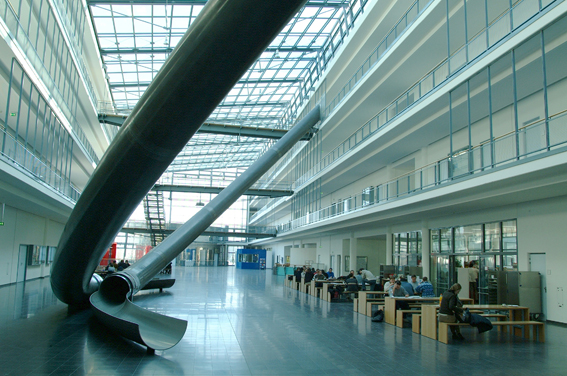
\includegraphics[width=0.5\textwidth]{figures/tum.jpg}
			%\caption{Example picture that was taken from an external source \takenFrom{asc_notes}.}
			%\label{fig:nodalBasis}
		%\end{figure}
		
		%References on figures work like this: blblablabla (see \refFigure{fig:nodalBasis}). If you used external knowledge for a paragraph, use the cite command at the very end of a sentence but right before the full stop \cite{ba_molzer}.
		
		%If you use an $l$ for math symbols, use $\ell$ instead for better readability.
		
	Vor dem Behandeln eines Problems ist es wichtig sich ebenso darüber zu informieren, was in diesem Bereich bereits in anderen Arbeiten behandelt wurde und welche Ergebnisse dabei erzielt wurden.
	\todo{Schönerer Einstieg!}
	Im Bereich der Benutzeroberflächen für Desktop-Computer gibt es zum Beispiel schon seit einigen Jahren Forschungen, welche sich mit der Platzierung und dem Design beschäftigen\todo{Fortsetzen und schöner machen}
	Auch mit der Platzierung in virtuellen 3D-Umgebungen haben sich einige Leute beschäftigt. \todo{Beispiele}
	Zu dem Thema plattformübergreifender Programme in der erweiterten Realität gibt es ebenso schon einige Ansätze \todo{Links}, aber diese verzichten häufig auf Benutzeroberflächen.
		
	\section{Priorisieren von Benutzeroberflächen}
		\todo{Abschnitt überprüfen und Beweise einfügen}
		Das Umstrukturieren von Menüs ist nicht trivial, denn jede Veränderung in der Benutzeroberfläche kann das Nutzererlebnis drastisch verändern. Dies ist sowohl in zweidimensionalen Programmen der Fall, wie auch in der virtuellen dreidimensionalen Welt. Mit diesem Nutzererlebnis setzt sich seit einigen Jahren der Bereich des UX Designs\todo{UX erklären} auseinander. Es gibt dabei allerdings keine perfekte Lösung, da es sich dabei um ein subjektives Erlebnis handelt\todo{Link zu UX 1}.
		Um aber das Risiko einer Verschlechterung des Nutzungserlebnisses gering zu halten, hilft es ... \todo{irgendwas mit Prioritätsstufen und Untermenüs}
		- UX
		- Prioritätsgruppen
		- Umsetzung in 2D
		
	\section{Positionierung in 2D}
		- Fenstergebunden WIMP
		- Menüs / Fenster
		- Bildschirmränder
		
	\section{Positionierung in 3D (VR/AR auch ohne)}
		- 3D Programm: UI in Welt platziert
		- Üblich Hände und Kopf 
		- Beispiele!
		- dreidimensionale Benutzeroberflächen